\section{Reproducibility details}
\label{app:repro}
\textbf{Harness and decoding.} Temperature 0 (greedy decoding; the default top-$p$ 0.95 and top-$k$ 64 are set but inactive), at most 4,608 output tokens per call, thinking budget 2,560 tokens, at most 34 tool calls and 44 turns per episode, 7.5 minutes per episode, 90 seconds per command.

\textbf{Serving.} Every arm is a LoRA adapter served with vLLM (\texttt{--enable-lora --max-loras 8 --max-cpu-loras 32 --max-lora-rank 32 --enable-prefix-caching --dtype bfloat16}). We serve the unedited model through an all-zero rank-16 adapter and request it by name like every other arm. At most 8 adapters were served together. In batches 6--15, all 8 arms of a batch were served together. Batches 3--5 (9--11 arms) were served as two groups. One group held the unedited model and the edits built on the base model. The other held our wave-5 RL adapter (\texttt{w5}) and the edits built on it. We compare each edit only with the unedited or RL arm of its own group. The \texttt{w5} runs of batches 3--5 were not served alongside the unedited arm, so \texttt{w5} minus unedited (32, 30, 36 against 28, 24, 22) is not a matched comparison (Appendix~\ref{app:prereg}). Rounds 2--5 served 6--8 adapters together. Concurrency is 4 per arm in development batches and 10 in the held-out tests.

\textbf{Commands.} \texttt{<port>} and \texttt{<checkpoint>} are placeholders. Building the always-on explore-more neuron at strength 0.25:
{\small\begin{verbatim}
python -m v2.steer.neuron build --tags edit@0 --layers 18,20,22 \
  --mode const --sign -1 --gain 4.0 --target 0.25 --ridge 0.001 --seed 0
\end{verbatim}}
The development-set evaluation script (\texttt{v2.eval.golden\_ab}) runs a development batch. It runs every arm of the batch on the 170 development tasks, with the arms served together. A held-out test:
{\small\begin{verbatim}
python -m v2.steer.confirm run --port <port> --rollouts 3 --concurrency 10
\end{verbatim}}

\textbf{Statistics.} Pure-Python scripts in the repository compute all statistics from saved per-task results (\texttt{scripts/review\_stats.py}, \texttt{stats.py}, \texttt{power.py}, \texttt{batch\_sd.py}, \texttt{consistency.py}, \texttt{cost\_per\_arm.py}, \texttt{make\_schedule\_table.py}, \texttt{selection\_null.py}, \texttt{shift\_check.py}, \texttt{passk.py}). \texttt{diag\_recompute/recompute.py} computes the diagnosis tallies. Mantel--Haenszel intervals use the Robins--Breslow--Greenland variance. Paired $t$ tests use the exact Student $t$ distribution through the incomplete beta function. Sign tests and McNemar tests are exact binomial and two-sided. Bootstrap intervals are paired percentile intervals over tasks with 10,000 resamples and seed 0. Cohen's $h$ is $2\arcsin\sqrt{p_1} - 2\arcsin\sqrt{p_2}$.

\textbf{Seeds.} Random controls of the always-on edit use seeds 0--2 (seed 1 in held-out Test 1); Claude's benchmark control uses seed 7. Activation splits are fixed.

\textbf{Compute.} Builds run on a CPU. Claude's round-1 builds took about 30--33 seconds per edit, and its later builds up to about 2 minutes (partly run in parallel). GPT's report records 20.8 seconds for its five edits. Each author session had a budget of 90 minutes of wall time on a CPU and no GPU. From the brief's creation to the author's last file write, the sessions took at least 19.9 (Claude), 14.4 (GPT) and 44.7 minutes (Gemini). The author sessions ran under coding-plan subscriptions, not per-token API billing. Evaluation took about 23 GPU-minutes per arm per 170-task run (batch GPU time divided by arms; mean batch wall-clock 2.2--2.8 hours). The runs behind the reported results took about 68 GPU-hours (development batches 3--16, benchmark batches 21--28, both held-out tests). All evaluation runs up to 2:35 PM ET on 12 November took about 108 GPU-hours. This total includes runs not reported here and the part of rounds 4 and 5 run by that time (\texttt{COMPUTE.md}).

\section{Batch schedule}
\label{app:schedule}
Tables~\ref{tab:schedule} and~\ref{tab:arenaschedule} list every arm of batches 3--15 and 21--28. Appendix~\ref{app:negative} describes the rank-16 batch (batch 16), and Appendix~\ref{app:followup} describes the later batches (29 onward). An edit's batch difference is its solved count minus the \texttt{base} count of the same batch. In batches 3--15, the always-on edit met a matched random control in batches 5, 6, 7, 10, 11, 12 and 13. These are 14 control runs of 4 adapters: one matched to strength 0.5 and three seeds matched to 0.25.

\begin{table}[h]
\caption{Schedule of development batches 3--15: every arm of every batch with its solved tasks of 170 (arm identifiers as in the released results). \texttt{base}: unedited model; \texttt{bneg\_t$s$}: always-on explore-more at strength $s$; \texttt{bnegmatch\_t0.5} and \texttt{bnm25\_s0}--\texttt{s2}: its matched random controls; \texttt{w5}: wave-5 RL adapter; \texttt{sub}, \texttt{bth}, \texttt{bsuc}, \texttt{vfyD}/\texttt{bvfyD}, \texttt{bedit}: submit-sooner, think-briefly, success, verify and edit-sooner edits; \texttt{p*}: prompt rules; \texttt{hp*}: constant-neuron rule edits; a name containing \texttt{match} is a control. A leading \texttt{b} (also \texttt{p*} and \texttt{hp*}) marks an arm built on the base model. In batches 3--5, the \texttt{econd}, \texttt{vfyD} and \texttt{sub} arms are built on \texttt{w5} and compared with \texttt{w5}. \texttt{w5} was not served alongside \texttt{base}, so \texttt{w5} minus \texttt{base} is not a matched comparison. \texttt{hp}$r$\texttt{18\_t}$s$: one constant neuron at layer 18, strength $s$, compiling the prompt rule $r$: \texttt{x} = read before the first edit (\texttt{pexp}), \texttt{e} = quote exactly and re-read after an edit (\texttt{pedit}), \texttt{b} = both (\texttt{pboth}) (Appendix~\ref{app:negative}). \texttt{bnegW} writes explore-more at five layers (10--26); \texttt{becond}, \texttt{econd}, \texttt{bse}, \texttt{bns}, \texttt{bn50\_th50} and \texttt{bcombo} are exploratory conditional or combined variants outside the main analysis.}
\label{tab:schedule}
\centering
\scriptsize
\resizebox{\linewidth}{!}{\begin{tabular}{rp{0.92\linewidth}}
\toprule
Batch & Arm: solved \\
\midrule
3 & \texttt{base}: 28; \texttt{becond\_t1.0}: 32; \texttt{bedit\_t0.5}: 22; \texttt{bedit\_t1.0}: 12; \texttt{beditmatch\_t1.0}: 25; \texttt{econd\_t0.5}: 30; \texttt{econd\_t1.0}: 27; \texttt{econdmatch\_t1.0}: 28; \texttt{w5}: 32 \\
4 & \texttt{base}: 24; \texttt{becond\_t1.0}: 26; \texttt{becondmatch\_t1.0}: 31; \texttt{bneg\_t0.5}: 28; \texttt{bneg\_t1.0}: 18; \texttt{bvfyD\_t1.0}: 24; \texttt{bvfyDmatch\_t1.0}: 27; \texttt{econd\_t1.0}: 24; \texttt{vfyD\_t1.0}: 17; \texttt{vfyDmatch\_t1.0}: 30; \texttt{w5}: 30 \\
5 & \texttt{base}: 22; \texttt{bneg\_t0.25}: 32; \texttt{bneg\_t0.5}: 31; \texttt{bnegmatch\_t0.5}: 27; \texttt{sub\_t0.25}: 33; \texttt{sub\_t0.5}: 26; \texttt{sub\_t1.0}: 27; \texttt{submatch\_t0.5}: 28; \texttt{w5}: 36 \\
6 & \texttt{base}: 29; \texttt{bneg\_t0.125}: 31; \texttt{bneg\_t0.25}: 29; \texttt{bneg\_t0.5}: 33; \texttt{bnegmatch\_t0.5}: 23; \texttt{bnm25\_s0}: 26; \texttt{bnm25\_s1}: 27; \texttt{bnm25\_s2}: 27 \\
7 & \texttt{base}: 22; \texttt{bneg\_t0.125}: 30; \texttt{bneg\_t0.25}: 30; \texttt{bneg\_t0.5}: 30; \texttt{bnegmatch\_t0.5}: 25; \texttt{bnm25\_s0}: 28; \texttt{bnm25\_s1}: 24; \texttt{bnm25\_s2}: 23 \\
8 & \texttt{base}: 29; \texttt{bcombo\_n25\_th50}: 26; \texttt{bn50\_th50}: 33; \texttt{bneg\_t0.5}: 26; \texttt{bth\_t0.25}: 28; \texttt{bth\_t0.5}: 28; \texttt{bth\_t1.0}: 25; \texttt{bthmatch\_t0.5}: 33 \\
9 & \texttt{base}: 27; \texttt{bneg\_t0.5}: 32; \texttt{bse\_t1.0}: 27; \texttt{bsematch\_t1.0}: 24; \texttt{bsuc\_t0.5}: 30; \texttt{bsuc\_t1.0}: 25; \texttt{bsuc\_t2.0}: 25; \texttt{bsucmatch\_t1.0}: 26 \\
10 & \texttt{base}: 26; \texttt{bnegW\_t0.25}: 27; \texttt{bneg\_t0.125}: 28; \texttt{bneg\_t0.25}: 31; \texttt{bneg\_t0.5}: 30; \texttt{bnm25\_s0}: 27; \texttt{bsuc\_t0.5}: 29; \texttt{bvfyD\_t0.25}: 24 \\
11 & \texttt{base}: 25; \texttt{bneg\_t0.25}: 29; \texttt{bneg\_t0.5}: 24; \texttt{bnegmatch\_t0.5}: 25; \texttt{bnm25\_s1}: 25; \texttt{bns\_n25\_s50}: 26; \texttt{bns\_n50\_s50}: 29; \texttt{bsuc\_t0.5}: 23 \\
12 & \texttt{base}: 27; \texttt{becond\_t1.0}: 28; \texttt{bn50\_th50}: 31; \texttt{bneg\_t0.125}: 33; \texttt{bneg\_t0.25}: 26; \texttt{bnm25\_s2}: 25; \texttt{bns\_n25\_s50}: 24; \texttt{bsucmatch\_t1.0}: 31 \\
13 & \texttt{base}: 30; \texttt{bneg\_t0.5}: 28; \texttt{bnm25\_s0}: 26; \texttt{pboth\_base}: 30; \texttt{pboth\_bneg\_t0.5}: 27; \texttt{pedit\_base}: 29; \texttt{pedit\_bneg\_t0.5}: 28; \texttt{pexp\_base}: 25 \\
14 & \texttt{base}: 28; \texttt{bneg\_t0.5}: 27; \texttt{hpb18\_t3}: 31; \texttt{hpe18\_t1}: 27; \texttt{hpe18\_t3}: 25; \texttt{hpe18\_t6}: 25; \texttt{hpematch\_t3}: 23; \texttt{hpx18\_t3}: 28 \\
15 & \texttt{base}: 25; \texttt{bneg\_t0.25}: 27; \texttt{hpb18\_t6}: 30; \texttt{hpe18\_t3}: 24; \texttt{hpx18\_t1}: 30; \texttt{hpx18\_t3}: 26; \texttt{hpx18\_t6}: 29; \texttt{hpxmatch\_t3}: 23 \\
\bottomrule
\end{tabular}}
\end{table}

\begin{table}[h]
\caption{Schedule of the three-author benchmark: solved tasks of 170 per arm and batch; an empty cell means the arm was not in that batch. Batches 21--23 are the screening batches, and 24--28 are the replication batches. The last six rows have these arm identifiers in the released results, in order: \texttt{ag\_think\_start\_explore\_ctrl}, \texttt{am\_damped\_dual\_explore\_concise}, its \texttt{\_ctrl}, \texttt{am\_hybrid\_explore\_verify\_guard}, \texttt{am\_oproj\_onesided\_commit\_damper}, \texttt{am\_whitened\_cond\_rushed\_read}. Claude's and GPT's controls were not run in batches 25 and 27, so for their repeated edits edit minus unedited uses six batches and edit minus control four.}
\label{tab:arenaschedule}
\centering
\footnotesize
\begin{tabular}{lrrrrrrrr}
\toprule
Arm & 21 & 22 & 23 & 24 & 25 & 26 & 27 & 28 \\
\midrule
Unedited model & 29 & 24 & 21 & 27 & 28 & 22 & 25 & 26 \\
Claude: always-on, 0.125 &  & 27 &  &  &  &  &  &  \\
Claude: before-first-edit gate &  & 33 &  & 29 & 31 & 31 & 30 & 28 \\
Claude: generated-positions gate &  & 25 &  &  &  &  &  &  \\
Claude: early-calls gate &  & 30 &  & 29 & 28 & 31 & 32 & 30 \\
Claude: random control &  & 25 &  & 28 &  & 26 &  & 27 \\
GPT: decision-token gate & 28 &  &  &  &  &  &  &  \\
GPT: decision-token gate + rotation & 33 &  &  & 27 & 30 & 30 & 27 & 24 \\
GPT: re-check after error & 27 &  &  &  &  &  &  &  \\
GPT: rank-two rotation & 28 &  &  &  &  &  &  &  \\
GPT: random control & 28 &  &  & 24 &  & 28 &  & 26 \\
Gemini: explore + concise, damped &  &  & 28 &  & 31 &  & 32 &  \\
Gemini: random control &  &  & 29 &  & 25 &  & 29 &  \\
Gemini: explore + submit guard &  &  & 27 &  &  &  &  &  \\
Gemini: attention-output damper &  &  & 25 &  &  &  &  &  \\
Gemini: rushed-edit $\rightarrow$ read gate &  &  & 24 &  &  &  &  &  \\
\bottomrule
\end{tabular}
\end{table}


\section{Prediction calibration}
\label{app:calib}
Table~\ref{tab:calib} lists all 15 pre-run predictions of \S\ref{sec:arena}, controls included. Each author's five arms share one unedited run, so the 15 outcomes are correlated. Gemini's batch had the lowest unedited count of the eight (21), and all five of its adapters landed above their point predictions.

\begin{table}[h]
\caption{Predicted change in solved tasks of 170 against the unedited model of the same batch (point and 80\% interval, written before the run) and the first-run outcome. ``In'' marks an outcome inside the interval.}
\label{tab:calib}
\centering
\footnotesize
\begin{tabular}{llrrrrrl}
\toprule
Author & Edit & Point & 80\% interval & Width & Solved & $\Delta$ & In \\
\midrule
Claude & always-on, 0.125 & $+1.5$ & $[-3, +6]$ & 9 & 27 & $+3$ & yes \\
(unedited 24) & before-first-edit gate & $+1.0$ & $[-4, +6]$ & 10 & 33 & $+9$ & no \\
 & generated-positions gate & $+0.5$ & $[-5, +6]$ & 11 & 25 & $+1$ & yes \\
 & early-calls gate & $0.0$ & $[-6, +5]$ & 11 & 30 & $+6$ & no \\
 & random control & $-0.5$ & $[-5, +3]$ & 8 & 25 & $+1$ & yes \\
\midrule
GPT & decision-token gate & $+2.0$ & $[-5, +9]$ & 14 & 28 & $-1$ & yes \\
(unedited 29) & gate + rotation & $+1.5$ & $[-7, +10]$ & 17 & 33 & $+4$ & yes \\
 & re-check after error & $+0.5$ & $[-6, +7]$ & 13 & 27 & $-2$ & yes \\
 & rank-two rotation & $+0.5$ & $[-6, +7]$ & 13 & 28 & $-1$ & yes \\
 & random control & $0.0$ & $[-6, +6]$ & 12 & 28 & $-1$ & yes \\
\midrule
Gemini & explore + concise, damped & $+3.8$ & $[-1.5, +9.0]$ & 10.5 & 28 & $+7$ & yes \\
(unedited 21) & attention-output damper & $+3.0$ & $[-3.0, +9.0]$ & 12 & 25 & $+4$ & yes \\
 & rushed-edit $\rightarrow$ read gate & $+2.6$ & $[-3.0, +8.5]$ & 11.5 & 24 & $+3$ & yes \\
 & explore + submit guard & $+2.3$ & $[-3.5, +8.0]$ & 11.5 & 27 & $+6$ & yes \\
 & random control & $-0.2$ & $[-5.0, +4.5]$ & 9.5 & 29 & $+8$ & no \\
\bottomrule
\end{tabular}
\end{table}

Mean interval width and mean absolute error of the point prediction, controls included: Claude 9.8 and 3.5; GPT 13.8 and 2.1; Gemini 11.0 and 3.3. Over the four edits alone the mean absolute error is 4.0 (Claude), 2.4 (GPT) and 2.1 (Gemini). The three misses are all outcomes above the interval, and one of them is a random control.

\section{Secondary statistics for the benchmark}
\label{app:stats}
The batch-level paired $t$ test is the primary analysis (\S\ref{sec:setting}). Table~\ref{tab:stats} adds the task-level analyses for the four repeated edits and their authors' controls. Task-level tests treat the 170 tasks as the unit and sum over batches.

\begin{table}[h]
\caption{Repeated edits of the benchmark. Batch level: mean difference in solved tasks of 170 per batch, its standard error (SE), paired $t$ and sign-test $p$ over batches. Task level: paired $t$ over tasks, exact McNemar $p$, paired bootstrap 95\% CI of the per-batch difference, Cohen's $h$. The task-level tests treat batches as fixed. Means are given to two decimals (Figure~\ref{fig:arena} rounds to one, e.g.\ $+1.8$ for Claude's control). Claude's and GPT's controls were not run in batches 25 and 27, so their edit-minus-unedited rows use six batches and their edit-minus-control rows four (three, batches 24, 26 and 28, in the replication-only rows, whose task-level columns are not computed).}
\label{tab:stats}
\centering
\scriptsize
\resizebox{\linewidth}{!}{\begin{tabular}{lrrrrrrrlr}
\toprule
 & & \multicolumn{4}{c}{Batch level} & \multicolumn{4}{c}{Task level} \\
\cmidrule(lr){3-6} \cmidrule(lr){7-10}
Comparison & Batches & Mean & SE & $t$ $p$ & Sign $p$ & $t$ $p$ & McNemar $p$ & 95\% CI & $h$ \\
\midrule
\multicolumn{10}{l}{\emph{Edit minus unedited model}} \\
Claude before-first-edit gate & 6 & $+5.00$ & 1.34 & 0.014 & 0.031 & 0.010 & 0.002 & $[1.33, 8.83]$ & 0.080 \\
\quad replication batches only & 5 & $+4.20$ & 1.32 & 0.033 & 0.063 & 0.046 & 0.020 & $[0.2, 8.4]$ & 0.067 \\
Claude early-calls gate & 6 & $+4.67$ & 1.36 & 0.019 & 0.063 & 0.044 & 0.009 & $[0.33, 9.33]$ & 0.074 \\
GPT gate + rotation & 6 & $+2.33$ & 1.41 & 0.158 & 0.375 & 0.187 & 0.198 & $[-1.0, 5.83]$ & 0.037 \\
Gemini explore + concise & 3 & $+5.67$ & 1.33 & 0.051 & 0.25 & 0.032 & 0.016 & $[0.67, 11.0]$ & 0.091 \\
\midrule
\multicolumn{10}{l}{\emph{Control minus unedited model}} \\
Claude control (ungated, 0.125 gap) & 4 & $+1.75$ & 0.75 & 0.10 & 0.125 & 0.44 & 0.435 & $[-2.5, 6.5]$ & 0.029 \\
GPT control & 4 & $+0.50$ & 1.94 & 0.81 & 1.0 & 0.80 & 0.89 & $[-3.25, 4.25]$ & 0.008 \\
Gemini control & 3 & $+3.00$ & 3.22 & 0.45 & 1.0 & 0.23 & 0.23 & $[-2.0, 8.0]$ & 0.049 \\
\midrule
\multicolumn{10}{l}{\emph{Edit minus its author's control}} \\
Claude before-first-edit gate & 4 & $+3.75$ & 1.70 & 0.11 & 0.125 & 0.128 & 0.082 & $[-1.0, 8.75]$ & 0.059 \\
\quad replication batches only & 3 & $+2.33$ & 1.33 & 0.22 & 0.25 & -- & -- & -- & -- \\
Claude early-calls gate & 4 & $+3.50$ & 0.96 & 0.035 & 0.125 & 0.213 & 0.125 & $[-2.0, 9.0]$ & 0.055 \\
\quad replication batches only & 3 & $+3.00$ & 1.15 & 0.12 & 0.25 & -- & -- & -- & -- \\
GPT gate + rotation & 4 & $+2.00$ & 1.47 & 0.267 & 0.625 & 0.384 & 0.382 & $[-2.5, 6.25]$ & 0.032 \\
Gemini explore + concise & 3 & $+2.67$ & 2.03 & 0.319 & 1.0 & 0.207 & 0.322 & $[-1.33, 6.67]$ & 0.042 \\
\bottomrule
\end{tabular}}
\end{table}

\textbf{Task-level counts.} Summed over batches, the before-first-edit gate did better than the unedited model on 22 tasks and worse on 12. Against its control, it did better on 21 and worse on 12 (sign test over tasks $p = 0.16$). The early-calls gate: 27 better, 15 worse than unedited. GPT's gate + rotation: 25 and 17. Gemini's edit: 19 and 10.

\textbf{Edits run once.} Difference from the unedited model of the batch, with task-level paired $t$ and exact McNemar $p$: Claude always-on $+3$ (0.47; 0.63); Claude generated-positions gate $+1$ (0.80; 1.0); GPT rank-two rotation $-1$ (0.83; 1.0); GPT re-check after error $-2$ (0.66; 0.82); GPT decision-token gate $-1$ (0.82; 1.0); Gemini explore + submit guard $+6$ (0.18; 0.26); Gemini attention-output damper $+4$ (0.25; 0.39); Gemini rushed-edit gate $+3$ (0.41; 0.58).

\textbf{Multiplicity.} Holm correction over the 12 screened edits, on task-level $p$ values: gate $0.010 \rightarrow 0.12$, Gemini's edit $0.032 \rightarrow 0.35$, early-calls gate $0.044 \rightarrow 0.44$, all others 1.0. These $p$ values use six batches (Gemini: three) for the four repeated edits and one batch for the other eight. Holm over the 12 screening batches alone (exact McNemar, one batch per edit): gate $0.035 \rightarrow 0.42$, every other edit 1.0. Among the four repeated edits, on replication batches only (batch-level $t$): gate $0.033 \rightarrow 0.13$, early-calls gate $0.054 \rightarrow 0.16$, Gemini's edit $0.24 \rightarrow 0.48$, GPT's edit $0.30 \rightarrow 0.48$. No comparison is significant at 0.05 after correction.

\begin{figure}[h]
\begin{center}
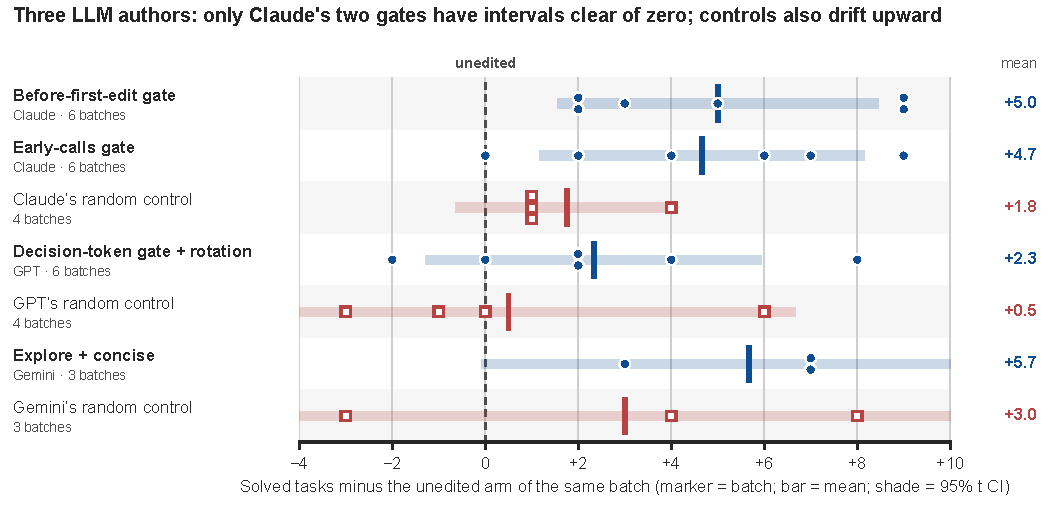
\includegraphics[width=1.0\linewidth]{figures/fig4_arena.pdf}
\end{center}
\caption{\textbf{Three-author benchmark.} Solved tasks of each repeated edit (blue) and each author's random control (red) minus the unedited arm of the same batch; one marker per batch, bar = mean, shade = 95\% $t$ interval of the mean. Only Claude's two gates have intervals that exclude zero, and no edit survives correction for the twelve screened (\S\ref{sec:arena}).}
\label{fig:arena}
\end{figure}

\subsection{Diagnosis tallies}
\label{app:diag}
\textbf{What the brief contained.} The three authors shared one brief. It stated lab-notebook rates for the unedited model and earlier results: 32\% of \texttt{edit\_file} calls fail (an earlier lab-notebook tally from batches 3--5; over the 13 unedited runs below the rate is 35\%); episodes with no failed edit solve 21\% against 4\% with one or more; the $N$th edit of an episode fails 14, 39, 49 and 60\% of the time; how episodes end (tests passed locally 64\%, never edited 17\%, tests errored 16\%); and the solved counts of earlier edits, including always-on explore-more. It gave no odds ratio, no reading-before-editing tally and no tally of calls before the first edit. Neither analysis below was in it. We computed the scripted analysis from a per-episode feature file written on 11 November, before the author sessions. Claude computed its tallies during its session.

\textbf{Scripted analysis} (2,720 episodes: 16 runs of the 170 tasks in batches 3--5, edited arms included; Mantel--Haenszel over tasks). Episodes with any failed edit: 54 of 988 solved against 355 of 1,732 without (odds ratio 0.27, $z = -6.9$, 54 informative tasks). Episodes with a completion of 2,500 tokens or more: 33 of 706 solved against 376 of 2,014 (odds ratio 0.34, $z = -4.6$, 47 tasks). On the three unedited runs alone (510 episodes) these odds ratios are 0.5 and 0.25, and the reading-before-first-edit odds ratio is 1.0.

\textbf{Claude's log} (13 unedited runs of batches 3--15, 2,210 episodes, 342 solved). The authoring model computed these tallies in its session and wrote them to \texttt{diag.log} and \texttt{diag2.log} in its work directory. We recomputed the edit-failure and calls-before-first-edit tallies independently from the saved trajectories and added 95\% intervals (\texttt{diag\_recompute/RESULT.md}). The recomputation reproduces every value, except for two episodes that the author's script put in the wrong failed-edit group. Of 4,916 \texttt{edit\_file} calls, 1,726 fail (35\%; 1,727 in our recomputation, part of the same two-episode discrepancy). The call right after a failed edit is \texttt{read\_file} in 37\% of cases and another \texttt{edit\_file} in 36\%. The next edit of the same file fails 82\% of the time without a re-read ($n = 741$) and 69\% with one ($n = 500$). Within-task odds ratios of solving: any failed edit 0.42; first edit failed 0.57. By number of calls before the first edit, the odds ratios are 0.76 for 0--2 calls, 1.42 for 3--4, 1.72 for 5--7 and 0.12 for 8 or more. Exploring longer is thus not monotonically better. The mean number of calls before the first edit is 4.8. We regenerated this last tally with the author's script (\texttt{diag2.py}) on the same 13 runs. The four bins hold 27\%, 34\%, 22\% and 17\% of episodes. The raw solve rate with versus without each bin is 0.283/0.107, 0.143/0.161, 0.113/0.166 and 0.027/0.181. The raw rate is highest for 0--2 calls because the model edits easy tasks quickly. Within task, the point estimates rise to 5--7 calls and fall at 8 or more; only the 8+ bin's interval excludes 1. The first-edit-failed odds ratio (0.57) and the re-read tallies are the author's values.
